\documentclass[twoside]{book}

% Packages required by doxygen
\usepackage{fixltx2e}
\usepackage{calc}
\usepackage{doxygen}
\usepackage[export]{adjustbox} % also loads graphicx
\usepackage{graphicx}
\usepackage[utf8]{inputenc}
\usepackage{makeidx}
\usepackage{multicol}
\usepackage{multirow}
\PassOptionsToPackage{warn}{textcomp}
\usepackage{textcomp}
\usepackage[nointegrals]{wasysym}
\usepackage[table]{xcolor}

% Font selection
\usepackage[T1]{fontenc}
\usepackage[scaled=.90]{helvet}
\usepackage{courier}
\usepackage{amssymb}
\usepackage{sectsty}
\renewcommand{\familydefault}{\sfdefault}
\allsectionsfont{%
  \fontseries{bc}\selectfont%
  \color{darkgray}%
}
\renewcommand{\DoxyLabelFont}{%
  \fontseries{bc}\selectfont%
  \color{darkgray}%
}
\newcommand{\+}{\discretionary{\mbox{\scriptsize$\hookleftarrow$}}{}{}}

% Page & text layout
\usepackage{geometry}
\geometry{%
  a4paper,%
  top=2.5cm,%
  bottom=2.5cm,%
  left=2.5cm,%
  right=2.5cm%
}
\tolerance=750
\hfuzz=15pt
\hbadness=750
\setlength{\emergencystretch}{15pt}
\setlength{\parindent}{0cm}
\setlength{\parskip}{3ex plus 2ex minus 2ex}
\makeatletter
\renewcommand{\paragraph}{%
  \@startsection{paragraph}{4}{0ex}{-1.0ex}{1.0ex}{%
    \normalfont\normalsize\bfseries\SS@parafont%
  }%
}
\renewcommand{\subparagraph}{%
  \@startsection{subparagraph}{5}{0ex}{-1.0ex}{1.0ex}{%
    \normalfont\normalsize\bfseries\SS@subparafont%
  }%
}
\makeatother

% Headers & footers
\usepackage{fancyhdr}
\pagestyle{fancyplain}
\fancyhead[LE]{\fancyplain{}{\bfseries\thepage}}
\fancyhead[CE]{\fancyplain{}{}}
\fancyhead[RE]{\fancyplain{}{\bfseries\leftmark}}
\fancyhead[LO]{\fancyplain{}{\bfseries\rightmark}}
\fancyhead[CO]{\fancyplain{}{}}
\fancyhead[RO]{\fancyplain{}{\bfseries\thepage}}
\fancyfoot[LE]{\fancyplain{}{}}
\fancyfoot[CE]{\fancyplain{}{}}
\fancyfoot[RE]{\fancyplain{}{\bfseries\scriptsize Generated by Doxygen }}
\fancyfoot[LO]{\fancyplain{}{\bfseries\scriptsize Generated by Doxygen }}
\fancyfoot[CO]{\fancyplain{}{}}
\fancyfoot[RO]{\fancyplain{}{}}
\renewcommand{\footrulewidth}{0.4pt}
\renewcommand{\chaptermark}[1]{%
  \markboth{#1}{}%
}
\renewcommand{\sectionmark}[1]{%
  \markright{\thesection\ #1}%
}

% Indices & bibliography
\usepackage{natbib}
\usepackage[titles]{tocloft}
\setcounter{tocdepth}{3}
\setcounter{secnumdepth}{5}
\makeindex

% Hyperlinks (required, but should be loaded last)
\usepackage{ifpdf}
\ifpdf
  \usepackage[pdftex,pagebackref=true]{hyperref}
\else
  \usepackage[ps2pdf,pagebackref=true]{hyperref}
\fi
\hypersetup{%
  colorlinks=true,%
  linkcolor=blue,%
  citecolor=blue,%
  unicode%
}

% Custom commands
\newcommand{\clearemptydoublepage}{%
  \newpage{\pagestyle{empty}\cleardoublepage}%
}

\usepackage{caption}
\captionsetup{labelsep=space,justification=centering,font={bf},singlelinecheck=off,skip=4pt,position=top}

%===== C O N T E N T S =====

\begin{document}

% Titlepage & ToC
\hypersetup{pageanchor=false,
             bookmarksnumbered=true,
             pdfencoding=unicode
            }
\pagenumbering{roman}
\begin{titlepage}
\vspace*{7cm}
\begin{center}%
{\Large My Project }\\
\vspace*{1cm}
{\large Generated by Doxygen 1.8.11}\\
\end{center}
\end{titlepage}
\clearemptydoublepage
\tableofcontents
\clearemptydoublepage
\pagenumbering{arabic}
\hypersetup{pageanchor=true}

%--- Begin generated contents ---
\chapter{Hierarchical Index}
\section{Class Hierarchy}
This inheritance list is sorted roughly, but not completely, alphabetically\+:\begin{DoxyCompactList}
\item \contentsline{section}{Fruit}{\pageref{classFruit}}{}
\begin{DoxyCompactList}
\item \contentsline{section}{Apple}{\pageref{classApple}}{}
\item \contentsline{section}{Grape}{\pageref{classGrape}}{}
\item \contentsline{section}{Orange}{\pageref{classOrange}}{}
\end{DoxyCompactList}
\item \contentsline{section}{List}{\pageref{classList}}{}
\item \contentsline{section}{List\+:\+:Node}{\pageref{structList_1_1Node}}{}
\end{DoxyCompactList}

\chapter{Class Index}
\section{Class List}
Here are the classes, structs, unions and interfaces with brief descriptions\+:\begin{DoxyCompactList}
\item\contentsline{section}{\hyperlink{structnode}{node} }{\pageref{structnode}}{}
\item\contentsline{section}{\hyperlink{structnode1}{node1} }{\pageref{structnode1}}{}
\item\contentsline{section}{\hyperlink{structnode__info}{node\+\_\+info} }{\pageref{structnode__info}}{}
\end{DoxyCompactList}

\chapter{File Index}
\section{File List}
Here is a list of all files with brief descriptions\+:\begin{DoxyCompactList}
\item\contentsline{section}{\hyperlink{Lab1_8c}{Lab1.\+c} }{\pageref{Lab1_8c}}{}
\end{DoxyCompactList}

\chapter{Class Documentation}
\hypertarget{classHindu}{}\section{Hindu Class Reference}
\label{classHindu}\index{Hindu@{Hindu}}


Inheritance diagram for Hindu\+:
\nopagebreak
\begin{figure}[H]
\begin{center}
\leavevmode
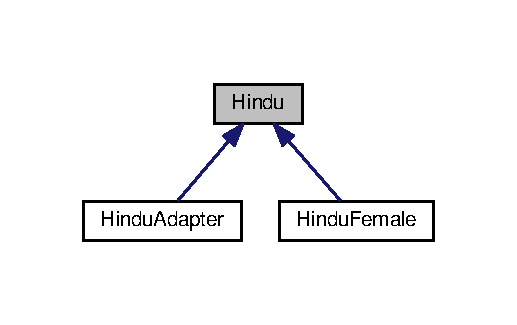
\includegraphics[width=248pt]{classHindu__inherit__graph}
\end{center}
\end{figure}
\subsection*{Public Member Functions}
\begin{DoxyCompactItemize}
\item 
virtual \hyperlink{classHindu_a01547b27ece449783df6c434a758afa2}{$\sim$\+Hindu} ()=default
\item 
virtual void \hyperlink{classHindu_aff8995fbde7a7c14940ed2fe2bf7b14c}{performs\+Hindu\+Ritual} () const =0
\end{DoxyCompactItemize}


\subsection{Constructor \& Destructor Documentation}
\index{Hindu@{Hindu}!````~Hindu@{$\sim$\+Hindu}}
\index{````~Hindu@{$\sim$\+Hindu}!Hindu@{Hindu}}
\subsubsection[{\texorpdfstring{$\sim$\+Hindu()=default}{~Hindu()=default}}]{\setlength{\rightskip}{0pt plus 5cm}virtual Hindu\+::$\sim$\+Hindu (
\begin{DoxyParamCaption}
{}
\end{DoxyParamCaption}
)\hspace{0.3cm}{\ttfamily [virtual]}, {\ttfamily [default]}}\hypertarget{classHindu_a01547b27ece449783df6c434a758afa2}{}\label{classHindu_a01547b27ece449783df6c434a758afa2}


\subsection{Member Function Documentation}
\index{Hindu@{Hindu}!performs\+Hindu\+Ritual@{performs\+Hindu\+Ritual}}
\index{performs\+Hindu\+Ritual@{performs\+Hindu\+Ritual}!Hindu@{Hindu}}
\subsubsection[{\texorpdfstring{performs\+Hindu\+Ritual() const =0}{performsHinduRitual() const =0}}]{\setlength{\rightskip}{0pt plus 5cm}virtual void Hindu\+::performs\+Hindu\+Ritual (
\begin{DoxyParamCaption}
{}
\end{DoxyParamCaption}
) const\hspace{0.3cm}{\ttfamily [pure virtual]}}\hypertarget{classHindu_aff8995fbde7a7c14940ed2fe2bf7b14c}{}\label{classHindu_aff8995fbde7a7c14940ed2fe2bf7b14c}


Implemented in \hyperlink{classHinduAdapter_a92390edb029c059347c8e3bdb825c5ce}{Hindu\+Adapter}, and \hyperlink{classHinduFemale_a7e5f4948f123a1a5e82f29f61e842c14}{Hindu\+Female}.



The documentation for this class was generated from the following file\+:\begin{DoxyCompactItemize}
\item 
\hyperlink{Adapter_8cpp}{Adapter.\+cpp}\end{DoxyCompactItemize}

\hypertarget{classHinduAdapter}{}\section{Hindu\+Adapter Class Reference}
\label{classHinduAdapter}\index{Hindu\+Adapter@{Hindu\+Adapter}}


Inheritance diagram for Hindu\+Adapter\+:
\nopagebreak
\begin{figure}[H]
\begin{center}
\leavevmode
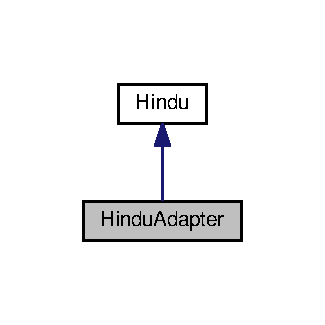
\includegraphics[width=156pt]{classHinduAdapter__inherit__graph}
\end{center}
\end{figure}


Collaboration diagram for Hindu\+Adapter\+:
\nopagebreak
\begin{figure}[H]
\begin{center}
\leavevmode
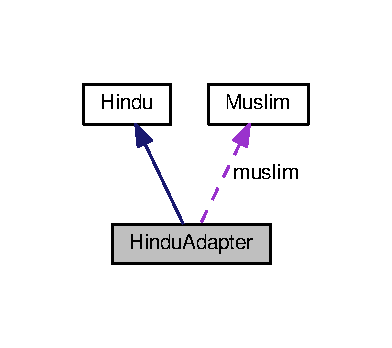
\includegraphics[width=188pt]{classHinduAdapter__coll__graph}
\end{center}
\end{figure}
\subsection*{Public Member Functions}
\begin{DoxyCompactItemize}
\item 
\hyperlink{classHinduAdapter_af378f4c2ad293836050be2b50821e781}{Hindu\+Adapter} (\hyperlink{classMuslim}{Muslim} $\ast$m)
\item 
virtual void \hyperlink{classHinduAdapter_a92390edb029c059347c8e3bdb825c5ce}{performs\+Hindu\+Ritual} () const override
\end{DoxyCompactItemize}
\subsection*{Private Attributes}
\begin{DoxyCompactItemize}
\item 
\hyperlink{classMuslim}{Muslim} $\ast$ \hyperlink{classHinduAdapter_a7447c22b644955b0ba076271ad4cb739}{muslim}
\end{DoxyCompactItemize}


\subsection{Constructor \& Destructor Documentation}
\index{Hindu\+Adapter@{Hindu\+Adapter}!Hindu\+Adapter@{Hindu\+Adapter}}
\index{Hindu\+Adapter@{Hindu\+Adapter}!Hindu\+Adapter@{Hindu\+Adapter}}
\subsubsection[{\texorpdfstring{Hindu\+Adapter(\+Muslim $\ast$m)}{HinduAdapter(Muslim *m)}}]{\setlength{\rightskip}{0pt plus 5cm}Hindu\+Adapter\+::\+Hindu\+Adapter (
\begin{DoxyParamCaption}
\item[{{\bf Muslim} $\ast$}]{m}
\end{DoxyParamCaption}
)\hspace{0.3cm}{\ttfamily [inline]}}\hypertarget{classHinduAdapter_af378f4c2ad293836050be2b50821e781}{}\label{classHinduAdapter_af378f4c2ad293836050be2b50821e781}

\begin{DoxyCode}
37 : \hyperlink{classHinduAdapter_a7447c22b644955b0ba076271ad4cb739}{muslim}(m) \{\}
\end{DoxyCode}


\subsection{Member Function Documentation}
\index{Hindu\+Adapter@{Hindu\+Adapter}!performs\+Hindu\+Ritual@{performs\+Hindu\+Ritual}}
\index{performs\+Hindu\+Ritual@{performs\+Hindu\+Ritual}!Hindu\+Adapter@{Hindu\+Adapter}}
\subsubsection[{\texorpdfstring{performs\+Hindu\+Ritual() const override}{performsHinduRitual() const override}}]{\setlength{\rightskip}{0pt plus 5cm}virtual void Hindu\+Adapter\+::performs\+Hindu\+Ritual (
\begin{DoxyParamCaption}
{}
\end{DoxyParamCaption}
) const\hspace{0.3cm}{\ttfamily [inline]}, {\ttfamily [override]}, {\ttfamily [virtual]}}\hypertarget{classHinduAdapter_a92390edb029c059347c8e3bdb825c5ce}{}\label{classHinduAdapter_a92390edb029c059347c8e3bdb825c5ce}


Implements \hyperlink{classHindu_aff8995fbde7a7c14940ed2fe2bf7b14c}{Hindu}.


\begin{DoxyCode}
38 \{\hyperlink{classHinduAdapter_a7447c22b644955b0ba076271ad4cb739}{muslim}->\hyperlink{classMuslim_af6792dc11aa3e0f86818af0c0ba4da11}{performsMuslimRitual}();\}
\end{DoxyCode}


Here is the call graph for this function\+:
\nopagebreak
\begin{figure}[H]
\begin{center}
\leavevmode
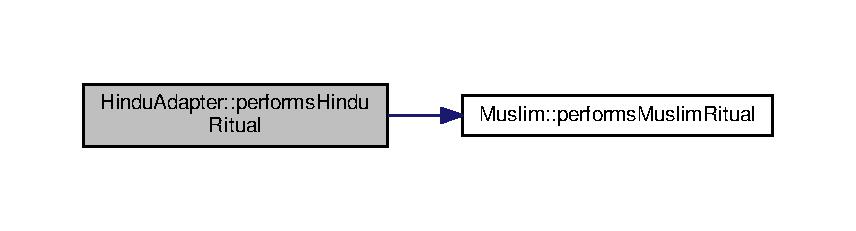
\includegraphics[width=350pt]{classHinduAdapter_a92390edb029c059347c8e3bdb825c5ce_cgraph}
\end{center}
\end{figure}




\subsection{Member Data Documentation}
\index{Hindu\+Adapter@{Hindu\+Adapter}!muslim@{muslim}}
\index{muslim@{muslim}!Hindu\+Adapter@{Hindu\+Adapter}}
\subsubsection[{\texorpdfstring{muslim}{muslim}}]{\setlength{\rightskip}{0pt plus 5cm}{\bf Muslim}$\ast$ Hindu\+Adapter\+::muslim\hspace{0.3cm}{\ttfamily [private]}}\hypertarget{classHinduAdapter_a7447c22b644955b0ba076271ad4cb739}{}\label{classHinduAdapter_a7447c22b644955b0ba076271ad4cb739}


The documentation for this class was generated from the following file\+:\begin{DoxyCompactItemize}
\item 
\hyperlink{Adapter_8cpp}{Adapter.\+cpp}\end{DoxyCompactItemize}

\hypertarget{classHinduFemale}{}\section{Hindu\+Female Class Reference}
\label{classHinduFemale}\index{Hindu\+Female@{Hindu\+Female}}


Inheritance diagram for Hindu\+Female\+:
\nopagebreak
\begin{figure}[H]
\begin{center}
\leavevmode
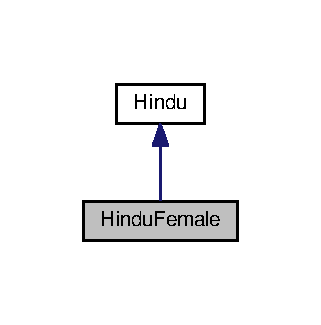
\includegraphics[width=154pt]{classHinduFemale__inherit__graph}
\end{center}
\end{figure}


Collaboration diagram for Hindu\+Female\+:
\nopagebreak
\begin{figure}[H]
\begin{center}
\leavevmode
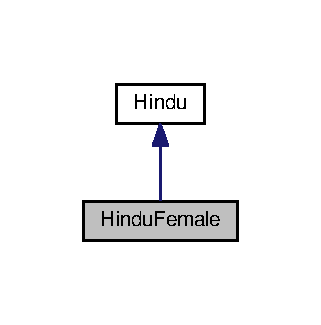
\includegraphics[width=154pt]{classHinduFemale__coll__graph}
\end{center}
\end{figure}
\subsection*{Public Member Functions}
\begin{DoxyCompactItemize}
\item 
virtual void \hyperlink{classHinduFemale_a7e5f4948f123a1a5e82f29f61e842c14}{performs\+Hindu\+Ritual} () const override
\end{DoxyCompactItemize}


\subsection{Member Function Documentation}
\index{Hindu\+Female@{Hindu\+Female}!performs\+Hindu\+Ritual@{performs\+Hindu\+Ritual}}
\index{performs\+Hindu\+Ritual@{performs\+Hindu\+Ritual}!Hindu\+Female@{Hindu\+Female}}
\subsubsection[{\texorpdfstring{performs\+Hindu\+Ritual() const override}{performsHinduRitual() const override}}]{\setlength{\rightskip}{0pt plus 5cm}virtual void Hindu\+Female\+::performs\+Hindu\+Ritual (
\begin{DoxyParamCaption}
{}
\end{DoxyParamCaption}
) const\hspace{0.3cm}{\ttfamily [inline]}, {\ttfamily [override]}, {\ttfamily [virtual]}}\hypertarget{classHinduFemale_a7e5f4948f123a1a5e82f29f61e842c14}{}\label{classHinduFemale_a7e5f4948f123a1a5e82f29f61e842c14}


Implements \hyperlink{classHindu_aff8995fbde7a7c14940ed2fe2bf7b14c}{Hindu}.


\begin{DoxyCode}
11 \{std::cout << \textcolor{stringliteral}{"Hindu girl performs Hindu ritual."} << std::endl;\}
\end{DoxyCode}


The documentation for this class was generated from the following file\+:\begin{DoxyCompactItemize}
\item 
\hyperlink{Adapter_8cpp}{Adapter.\+cpp}\end{DoxyCompactItemize}

\hypertarget{classHinduRitual}{}\section{Hindu\+Ritual Class Reference}
\label{classHinduRitual}\index{Hindu\+Ritual@{Hindu\+Ritual}}
\subsection*{Public Member Functions}
\begin{DoxyCompactItemize}
\item 
void \hyperlink{classHinduRitual_af83c2fe1551849f9e294f1e19a146ee9}{carry\+Out\+Ritual} (\hyperlink{classHindu}{Hindu} $\ast$hindu)
\end{DoxyCompactItemize}


\subsection{Member Function Documentation}
\index{Hindu\+Ritual@{Hindu\+Ritual}!carry\+Out\+Ritual@{carry\+Out\+Ritual}}
\index{carry\+Out\+Ritual@{carry\+Out\+Ritual}!Hindu\+Ritual@{Hindu\+Ritual}}
\subsubsection[{\texorpdfstring{carry\+Out\+Ritual(\+Hindu $\ast$hindu)}{carryOutRitual(Hindu *hindu)}}]{\setlength{\rightskip}{0pt plus 5cm}void Hindu\+Ritual\+::carry\+Out\+Ritual (
\begin{DoxyParamCaption}
\item[{{\bf Hindu} $\ast$}]{hindu}
\end{DoxyParamCaption}
)\hspace{0.3cm}{\ttfamily [inline]}}\hypertarget{classHinduRitual_af83c2fe1551849f9e294f1e19a146ee9}{}\label{classHinduRitual_af83c2fe1551849f9e294f1e19a146ee9}

\begin{DoxyCode}
27                                                \{
28                 std::cout << \textcolor{stringliteral}{"On with the Hindu rituals!"} << std::endl;
29                 hindu->\hyperlink{classHindu_aff8995fbde7a7c14940ed2fe2bf7b14c}{performsHinduRitual}();
30             \}
\end{DoxyCode}


Here is the call graph for this function\+:
\nopagebreak
\begin{figure}[H]
\begin{center}
\leavevmode
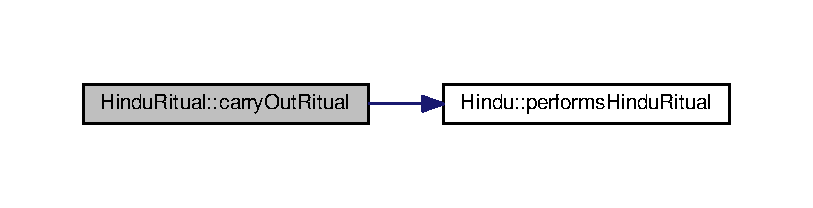
\includegraphics[width=350pt]{classHinduRitual_af83c2fe1551849f9e294f1e19a146ee9_cgraph}
\end{center}
\end{figure}




The documentation for this class was generated from the following file\+:\begin{DoxyCompactItemize}
\item 
\hyperlink{Adapter_8cpp}{Adapter.\+cpp}\end{DoxyCompactItemize}

\hypertarget{classMuslim}{}\section{Muslim Class Reference}
\label{classMuslim}\index{Muslim@{Muslim}}


Inheritance diagram for Muslim\+:
\nopagebreak
\begin{figure}[H]
\begin{center}
\leavevmode
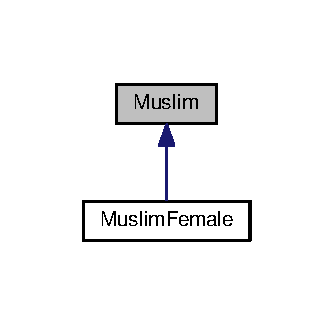
\includegraphics[width=160pt]{classMuslim__inherit__graph}
\end{center}
\end{figure}
\subsection*{Public Member Functions}
\begin{DoxyCompactItemize}
\item 
virtual \hyperlink{classMuslim_acaf81e854d0075f29f9d2d4d9ea12897}{$\sim$\+Muslim} ()=default
\item 
virtual void \hyperlink{classMuslim_af6792dc11aa3e0f86818af0c0ba4da11}{performs\+Muslim\+Ritual} () const =0
\end{DoxyCompactItemize}


\subsection{Constructor \& Destructor Documentation}
\index{Muslim@{Muslim}!````~Muslim@{$\sim$\+Muslim}}
\index{````~Muslim@{$\sim$\+Muslim}!Muslim@{Muslim}}
\subsubsection[{\texorpdfstring{$\sim$\+Muslim()=default}{~Muslim()=default}}]{\setlength{\rightskip}{0pt plus 5cm}virtual Muslim\+::$\sim$\+Muslim (
\begin{DoxyParamCaption}
{}
\end{DoxyParamCaption}
)\hspace{0.3cm}{\ttfamily [virtual]}, {\ttfamily [default]}}\hypertarget{classMuslim_acaf81e854d0075f29f9d2d4d9ea12897}{}\label{classMuslim_acaf81e854d0075f29f9d2d4d9ea12897}


\subsection{Member Function Documentation}
\index{Muslim@{Muslim}!performs\+Muslim\+Ritual@{performs\+Muslim\+Ritual}}
\index{performs\+Muslim\+Ritual@{performs\+Muslim\+Ritual}!Muslim@{Muslim}}
\subsubsection[{\texorpdfstring{performs\+Muslim\+Ritual() const =0}{performsMuslimRitual() const =0}}]{\setlength{\rightskip}{0pt plus 5cm}virtual void Muslim\+::performs\+Muslim\+Ritual (
\begin{DoxyParamCaption}
{}
\end{DoxyParamCaption}
) const\hspace{0.3cm}{\ttfamily [pure virtual]}}\hypertarget{classMuslim_af6792dc11aa3e0f86818af0c0ba4da11}{}\label{classMuslim_af6792dc11aa3e0f86818af0c0ba4da11}


Implemented in \hyperlink{classMuslimFemale_ab08e692639df1e16fc5d41b18cb01765}{Muslim\+Female}.



The documentation for this class was generated from the following file\+:\begin{DoxyCompactItemize}
\item 
\hyperlink{Adapter_8cpp}{Adapter.\+cpp}\end{DoxyCompactItemize}

\hypertarget{classMuslimFemale}{}\section{Muslim\+Female Class Reference}
\label{classMuslimFemale}\index{Muslim\+Female@{Muslim\+Female}}


Inheritance diagram for Muslim\+Female\+:
\nopagebreak
\begin{figure}[H]
\begin{center}
\leavevmode
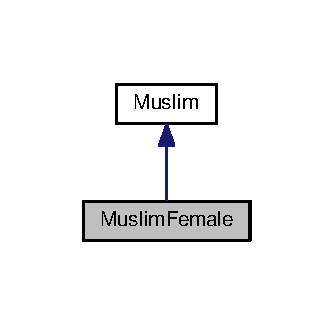
\includegraphics[width=160pt]{classMuslimFemale__inherit__graph}
\end{center}
\end{figure}


Collaboration diagram for Muslim\+Female\+:
\nopagebreak
\begin{figure}[H]
\begin{center}
\leavevmode
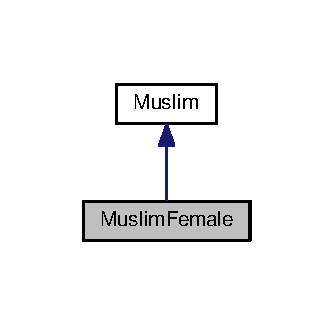
\includegraphics[width=160pt]{classMuslimFemale__coll__graph}
\end{center}
\end{figure}
\subsection*{Public Member Functions}
\begin{DoxyCompactItemize}
\item 
virtual void \hyperlink{classMuslimFemale_ab08e692639df1e16fc5d41b18cb01765}{performs\+Muslim\+Ritual} () const override
\end{DoxyCompactItemize}


\subsection{Member Function Documentation}
\index{Muslim\+Female@{Muslim\+Female}!performs\+Muslim\+Ritual@{performs\+Muslim\+Ritual}}
\index{performs\+Muslim\+Ritual@{performs\+Muslim\+Ritual}!Muslim\+Female@{Muslim\+Female}}
\subsubsection[{\texorpdfstring{performs\+Muslim\+Ritual() const override}{performsMuslimRitual() const override}}]{\setlength{\rightskip}{0pt plus 5cm}virtual void Muslim\+Female\+::performs\+Muslim\+Ritual (
\begin{DoxyParamCaption}
{}
\end{DoxyParamCaption}
) const\hspace{0.3cm}{\ttfamily [inline]}, {\ttfamily [override]}, {\ttfamily [virtual]}}\hypertarget{classMuslimFemale_ab08e692639df1e16fc5d41b18cb01765}{}\label{classMuslimFemale_ab08e692639df1e16fc5d41b18cb01765}


Implements \hyperlink{classMuslim_af6792dc11aa3e0f86818af0c0ba4da11}{Muslim}.


\begin{DoxyCode}
22 \{std::cout << \textcolor{stringliteral}{"Muslim girl performs Muslim ritual."} << std::endl;\}
\end{DoxyCode}


The documentation for this class was generated from the following file\+:\begin{DoxyCompactItemize}
\item 
\hyperlink{Adapter_8cpp}{Adapter.\+cpp}\end{DoxyCompactItemize}

\chapter{File Documentation}
\hypertarget{Adapter_8cpp}{}\section{Adapter.\+cpp File Reference}
\label{Adapter_8cpp}\index{Adapter.\+cpp@{Adapter.\+cpp}}
{\ttfamily \#include $<$iostream$>$}\\*
Include dependency graph for Adapter.\+cpp\+:
\nopagebreak
\begin{figure}[H]
\begin{center}
\leavevmode
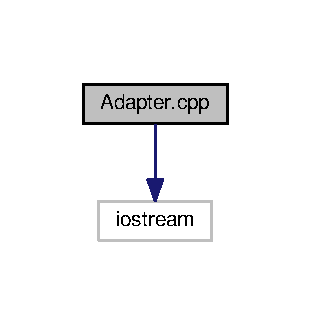
\includegraphics[width=149pt]{Adapter_8cpp__incl}
\end{center}
\end{figure}
\subsection*{Classes}
\begin{DoxyCompactItemize}
\item 
class \hyperlink{classHindu}{Hindu}
\item 
class \hyperlink{classHinduFemale}{Hindu\+Female}
\item 
class \hyperlink{classMuslim}{Muslim}
\item 
class \hyperlink{classMuslimFemale}{Muslim\+Female}
\item 
class \hyperlink{classHinduRitual}{Hindu\+Ritual}
\item 
class \hyperlink{classHinduAdapter}{Hindu\+Adapter}
\end{DoxyCompactItemize}
\subsection*{Functions}
\begin{DoxyCompactItemize}
\item 
int \hyperlink{Adapter_8cpp_ae66f6b31b5ad750f1fe042a706a4e3d4}{main} ()
\end{DoxyCompactItemize}


\subsection{Function Documentation}
\index{Adapter.\+cpp@{Adapter.\+cpp}!main@{main}}
\index{main@{main}!Adapter.\+cpp@{Adapter.\+cpp}}
\subsubsection[{\texorpdfstring{main()}{main()}}]{\setlength{\rightskip}{0pt plus 5cm}int main (
\begin{DoxyParamCaption}
{}
\end{DoxyParamCaption}
)}\hypertarget{Adapter_8cpp_ae66f6b31b5ad750f1fe042a706a4e3d4}{}\label{Adapter_8cpp_ae66f6b31b5ad750f1fe042a706a4e3d4}

\begin{DoxyCode}
41            \{  \textcolor{comment}{// Client code}
42     \hyperlink{classHinduFemale}{HinduFemale}* hinduGirl = \textcolor{keyword}{new} \hyperlink{classHinduFemale}{HinduFemale};
43     \hyperlink{classMuslimFemale}{MuslimFemale}* muslimGirl = \textcolor{keyword}{new} \hyperlink{classMuslimFemale}{MuslimFemale};
44     \hyperlink{classHinduRitual}{HinduRitual} hinduRitual;
45 \textcolor{comment}{//  hinduRitual.carryOutRitual (muslimGirl);  // Will not compile of course since the parameter must be of
       type Hindu*.}
46     \hyperlink{classHinduAdapter}{HinduAdapter}* adaptedMuslim = \textcolor{keyword}{new} \hyperlink{classHinduAdapter}{HinduAdapter} (muslimGirl);  \textcolor{comment}{// muslimGirl has
       adapted to become a Hindu!}
47     
48     hinduRitual.\hyperlink{classHinduRitual_af83c2fe1551849f9e294f1e19a146ee9}{carryOutRitual} (hinduGirl);
49     hinduRitual.\hyperlink{classHinduRitual_af83c2fe1551849f9e294f1e19a146ee9}{carryOutRitual} (adaptedMuslim);  \textcolor{comment}{// So now muslimGirl, in the form of
       adaptedMuslim, participates in the hinduRitual!}
50                 \textcolor{comment}{// Note that muslimGirl is carrying out her own type of ritual in hinduRitual though.}
51     
52     \textcolor{keyword}{delete} adaptedMuslim;  \textcolor{comment}{// adaptedMuslim is not needed anymore}
53     \textcolor{keyword}{delete} muslimGirl; \textcolor{comment}{// muslimGirl is not needed anymore}
54         \textcolor{keyword}{delete} hinduGirl; \textcolor{comment}{// hinduGirl is not needed anymore, too}
55     \textcolor{keywordflow}{return} 0;
56 \}\end{DoxyCode}


Here is the call graph for this function\+:
\nopagebreak
\begin{figure}[H]
\begin{center}
\leavevmode
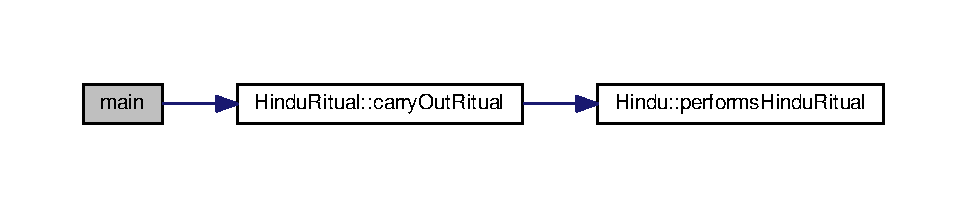
\includegraphics[width=350pt]{Adapter_8cpp_ae66f6b31b5ad750f1fe042a706a4e3d4_cgraph}
\end{center}
\end{figure}



%--- End generated contents ---

% Index
\backmatter
\newpage
\phantomsection
\clearemptydoublepage
\addcontentsline{toc}{chapter}{Index}
\printindex

\end{document}
